\documentclass{article}
\usepackage[utf8]{inputenc}
\usepackage[a4paper, total={6in, 8.5in}]{geometry}
\usepackage{indentfirst}
\usepackage{fancyvrb}
\usepackage{array}
\usepackage{graphicx}
\usepackage{float}

\usepackage{caption}
\usepackage{subcaption}

\title{Advanced programming for HPC}
\author{Minh Long PHAM - M21.ICT.008}
\date{December 2022}

\begin{document}

\maketitle

\section{Hardware}
The following hardwares were used to do the labwork:
\begin{itemize}
    \item CPU: Intel Core i5-8250U 
    \item GPU: NVIDIA GeForce MX130
\end{itemize}

\section{Implementation}
The steps to do the labwork:
\begin{itemize}
    \item Load an RGB image to an multidimensional array, which has the shape of (height, width, 3).
    \item Reshape the array's shape to (height*width, 3) for easier implementation.
    \item Feed the array to the functions to transform RGB image to an image in grayscale using manual method with CPU and CUDA with GPU.
    \item Save images and compare the implementation duration between two functions.
\end{itemize}

\begin{figure}[H]
    \center{
        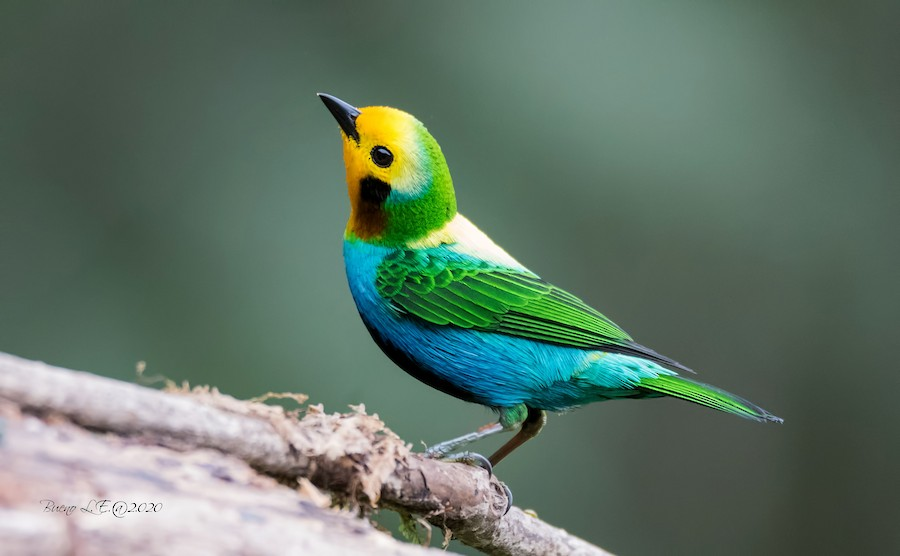
\includegraphics[scale=0.3]{images/bird.png}
    }
    \caption{Sample image}
\end{figure}

\begin{figure}[H]
\centering
\begin{subfigure}{.5\textwidth}
  \centering
  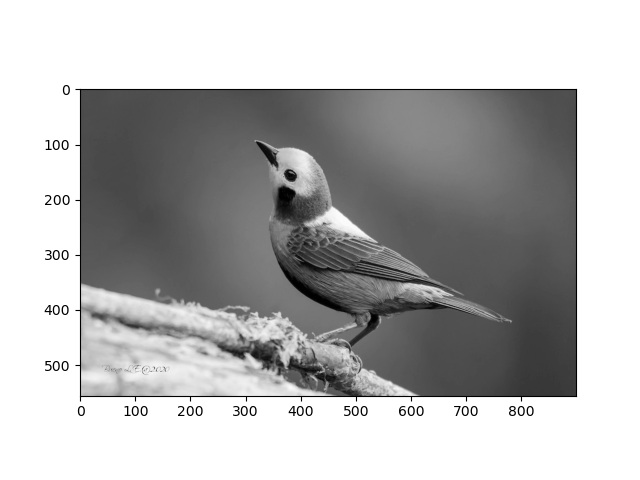
\includegraphics[scale=0.45]{images/lw3manual.png}
  \caption{Grayscale image by CPU}
  \label{fig:sub1}
\end{subfigure}%
\begin{subfigure}{.5\textwidth}
  \centering
  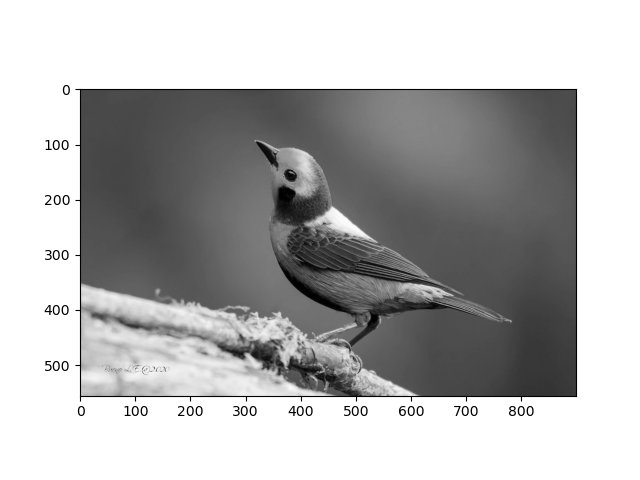
\includegraphics[scale=0.45]{images/lw3cuda.png}
  \caption{Grayscale image by GPU}
  \label{fig:sub2}
\end{subfigure}
\label{fig:test}
\end{figure}

Regarding the benchmark, I only measured the time to execute the main function transformimg a RGB image to a grayscale one. In the case which the block size is 64, the execution time using GPU is nearly 10 times faster than that duration using CPU.

\begin{figure}[H]
    \center{
        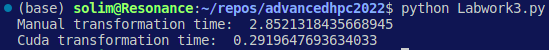
\includegraphics[scale=0.7]{images/collapsedtime.png}
    }
    \caption{Result with a block size of 64}
\end{figure}

Since the implementation time varies each time the code is executed, I took the average time of three execution times for each block size experiment. Block sizes of 16, 32, 64, 128, 256 and 1024 were used to do the comparison. It seems that the block sizes from 64 to 256 achieve optimal run time but overall the execution time is not affected so much by block size value.

\begin{figure}[H]
    \center{
        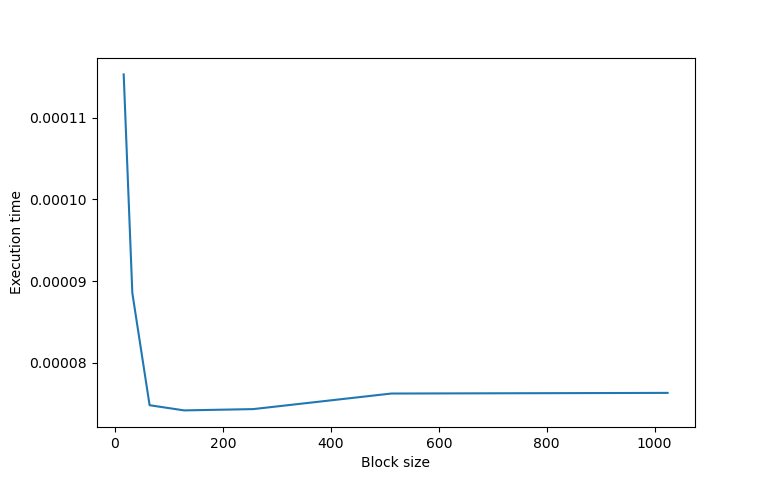
\includegraphics[scale=0.5]{images/compare.png}
    }
    \caption{Comparison between various block sizes}
\end{figure}

\end{document}
